
% This LaTeX was auto-generated from an M-file by MATLAB.
% To make changes, update the M-file and republish this document.

\documentclass{article}
\usepackage{graphicx}
\usepackage{color}

\sloppy
\definecolor{lightgray}{gray}{0.5}
\setlength{\parindent}{0pt}

\begin{document}

    
    
\subsection*{Contents}

\begin{itemize}
\setlength{\itemsep}{-1ex}
   \item Ejercicio 3
   \item Ejercicio 3.1
   \item mipca.m
   \item Ejercicio 3.2
   \item mezclar.m
   \item Ejercicio 3.3
\end{itemize}


\subsection*{Ejercicio 3}

\begin{par}
Análisis estadístico de datos - PCA.
\end{par} \vspace{1em}
\begin{verbatim}
clc; close all; clear all;
\end{verbatim}


\subsection*{Ejercicio 3.1}

\begin{par}
Implemente el algoritmo de PCA.
\end{par} \vspace{1em}
\begin{par}
Debajo se copia el código fuente de la función implementada. La descripción de la misma se encuentra dentro del código.
\end{par} \vspace{1em}


\subsection*{mipca.m}

\begin{verbatim}
dbtype mipca.m
\end{verbatim}

        \color{lightgray} \begin{verbatim}
1     function [PC, autoval] = mipca( X )
2     %MIPCA devuelve la matriz que permite proyectar los datos X sobre las
3     %direcciones obtenidas por medio del análisis de componentes principales.
4     % X es una matriz de D por N, donde cada observación se acomoda como
5     % columna. D es la dimensión de cada observación y N es el
6     % número total de observaciones.
7     %
8     % PC es la matriz de transformación de la base original a las direcciones
9     % principales. Las columnas son los versores de la nueva base.
10    %
11    % autoval es un vector con los autovalores asociados a PC, en orden 
12    % decreciente.
13    
14    % Matriz de covarianza (internamente realiza la resta de la media)
15    S = cov(X'); % traspongo para que tome bien las observaciones
16    
17    % Obtengo la matriz de autovectores y una matriz con los autovalores de S
18    [autovec, autoval] = eig(S);
19    
20    % Ordeno la matriz de transformación por orden descendente de autovalores
21    PC = fliplr(autovec);
22    
23    % Autovalores ordenados por módulo decreciente
24    autoval = flipdim(diag(autoval),1);
25    
26    end
27    

\end{verbatim} \color{black}
    

\subsection*{Ejercicio 3.2}

\begin{par}
Escriba un programa que le permita generar datos aleatorios $\mathbf(x)$ a partir del siguiente modelo generativo lineal: $\mathbf(x) = \mathbf(A) \mathbf(s)$, donde $\mathbf(s)$ es el vector de fuentes (aleatorio) y $\mathbf(A)$ es la matriz de mezcla.
\end{par} \vspace{1em}
\begin{par}
Debajo se copia el código fuente de la función implementada. La descripción de la misma se encuentra dentro del código.
\end{par} \vspace{1em}


\subsection*{mezclar.m}

\begin{verbatim}
dbtype mezclar.m
\end{verbatim}

        \color{lightgray} \begin{verbatim}
1     function X = mezclar( A, s1, s2 )
2     %MEZCLAR X = ( A, s1, s2 ) dada la matriz de mecla A y las fuentes s1 y s2 
3     % (vectores) se generan dos mezclas x1 y x2 (cada una en un renglón de X).
4     
5     if size(s1,1) ~= 1
6         s1 = s1'; % convierte s1 en un vector horizontal si no lo es
7     end
8     if size(s2,1) ~= 1
9         s2 = s2'; % convierte s2 en un vector horizontal si no lo es
10    end
11    
12    S = vertcat(s1,s2);
13    X = A * S;
14    end
15    

\end{verbatim} \color{black}
    

\subsection*{Ejercicio 3.3}

\begin{par}
A partir de datos de dos mezclas, obtenidos mediante dos fuentes y una matriz de mezcla aleatoria, utilice PCA para lo siguiente:
\end{par} \vspace{1em}
\begin{enumerate}
\setlength{\itemsep}{-1ex}
   \item Pruebe con fuentes con distribución gaussiana y laplaciana, para matrices de mezcla con columnas ortogonales y no ortogonales.
   \item Para cada caso de los anteriores y cada etapa (fuentes, mezclas, señales separadas) dibuje un gráfico de dispersión de las variables.
   \item Luego de la separación obtenga la matriz $\mathbf{W}$ correspondiente.
\end{enumerate}
\begin{verbatim}
N = 300;

% Fuentes gaussianas y laplacianas
s{1} = randgauss1D(1, 1, N)';
s{2} = randgauss1D(3, 3, N)';
s{3} = randlap(N, 2 ,2)';
s{4} = randlap(N, 5 ,0.9)';
s{5} = randgauss1D(1, 1, N)';
s{6} = randlap(N, 2 ,2)';

% Se corroboran los signos para impedir que ambas mezclas sean
% proporcionales
signos = ones(2);
while isequal(signos(1,:),signos(2,:)) || isequal(signos(1,:), -signos(2,:))
    signos = sign(rand(2)-0.5);
end

% Generacion aleatoria de las matrices de mezcla
A{1} = repmat(2*rand(1,2)-1,2,1) .* signos;% Mezcla con columnas ortogonales
A{2} = (2*rand(2)-1) .* signos;            % Mezcla no ortogonal
titort{1} = 'ortogonales';
titort{2} = 'no ortogonales';
suptit{1} = 'Fuentes gaussianas';
suptit{2} = 'Fuentes laplacianas';
suptit{3} = 'Fuente gaussiana y laplaciana';

for ss = 1:3
    figure
    for aa = 1:2
        X = mezclar(A{aa},s{2*ss-1},s{2*ss}); % Mezcla las señales
        x1m = mean(X(1,:)); % media de la primera dimension
        x2m = mean(X(2,:)); % media de la segunda dimension

        W = mipca(X); % Obtengo la Matriz de Proyección de X sobre las
                      % direcciones principales, versores por columnas

        Y = W' * X; % Proyecto los datos sobre las direcciones principales
        % y_1  = w_11 * x_1 + w_21 * x_2
        % y_2  = w_12 * x_2 + w_22 * x_2

        subplot(2,3,1+3*(aa-1))
        scatter(s{2*ss-1}, s{2*ss}); axis equal;
        title({'Fuentes';['columnas ' titort{aa}]} )
        xlabel('s_1'); ylabel('s_2');

        subplot(2,3,2+3*(aa-1))
        scatter(X(1,:), X(2,:)); axis equal;
        hold on;
        plot(x1m + [0 5*W(1,1)],x2m + [0 5*W(2,1)], 'k','LineWidth',2)
        plot(x1m + [0 5*W(1,2)],x2m + [0 5*W(2,2)], 'k','LineWidth',2)
        hold off
        title({'Mezclas';['columnas ' titort{aa}]} )
        xlabel('x_1'); ylabel('x_2');

        subplot(2,3,3+3*(aa-1))
        scatter(Y(1,:), Y(2,:)); axis equal;
        title({'Señales separadas';['columnas ' titort{aa}]} )
        xlabel('y_1'); ylabel('y_2');

        Ainv  = inv(A{aa});
        disp([suptit{ss} ', columnas ' titort{aa}])
        fprintf(['A = [%0.2f %0.2f],\t Ainv = [%0.2f %0.2f],\t W = [%0.2f %0.2f]\n'...
                 '    [%0.2f %0.2f],\t Ainv = [%0.2f %0.2f],\t     [%0.2f %0.2f]\n\n'],...
                 A{aa}(1,:), Ainv(2,:), W(1,:), A{aa}(2,:), Ainv(2,:), W(2,:) );
    end
    suptitle(suptit{ss})
end
\end{verbatim}

        \color{lightgray} \begin{verbatim}Fuentes gaussianas, columnas ortogonales
A = [-0.20 0.82],	 Ainv = [0.61 -0.61],	 W = [-0.70 -0.71]
    [-0.20 -0.82],	 Ainv = [0.61 -0.61],	     [0.71 -0.70]

Fuentes gaussianas, columnas no ortogonales
A = [0.45 -0.19],	 Ainv = [-1.78 0.86],	 W = [-0.13 -0.99]
    [0.92 0.78],	 Ainv = [-1.78 0.86],	     [0.99 -0.13]

Fuentes laplacianas, columnas ortogonales
A = [-0.20 0.82],	 Ainv = [0.61 -0.61],	 W = [-0.72 -0.69]
    [-0.20 -0.82],	 Ainv = [0.61 -0.61],	     [0.69 -0.72]

Fuentes laplacianas, columnas no ortogonales
A = [0.45 -0.19],	 Ainv = [-1.78 0.86],	 W = [0.38 -0.93]
    [0.92 0.78],	 Ainv = [-1.78 0.86],	     [0.93 0.38]

Fuente gaussiana y laplaciana, columnas ortogonales
A = [-0.20 0.82],	 Ainv = [0.61 -0.61],	 W = [-0.70 -0.71]
    [-0.20 -0.82],	 Ainv = [0.61 -0.61],	     [0.71 -0.70]

Fuente gaussiana y laplaciana, columnas no ortogonales
A = [0.45 -0.19],	 Ainv = [-1.78 0.86],	 W = [-0.13 -0.99]
    [0.92 0.78],	 Ainv = [-1.78 0.86],	     [0.99 -0.13]

\end{verbatim} \color{black}
    
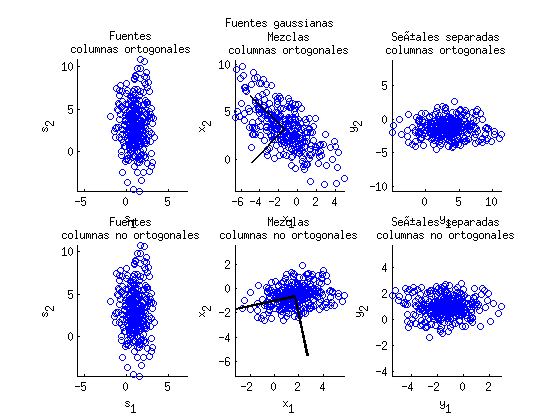
\includegraphics [width=4in]{Ejercicio3_01.png}

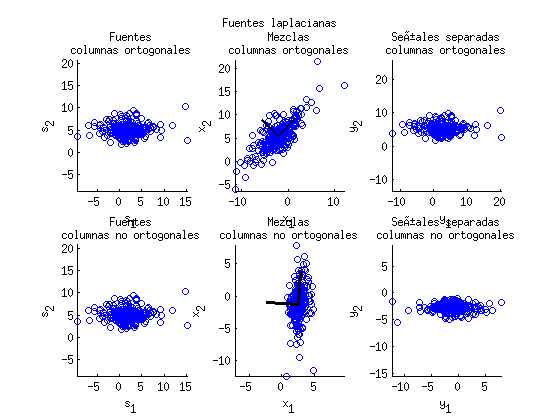
\includegraphics [width=4in]{Ejercicio3_02.png}

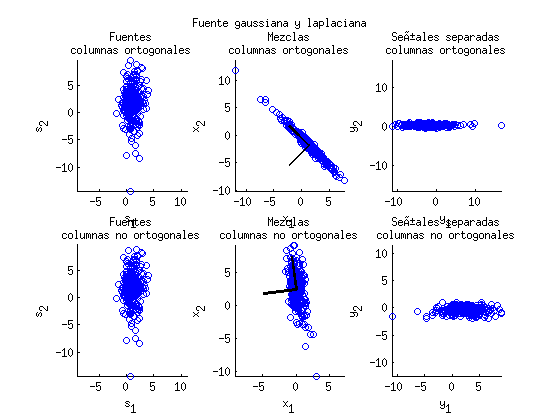
\includegraphics [width=4in]{Ejercicio3_03.png}
\begin{par}
En las figuras \ensuremath{\backslash}ref\{....\} se muestra cada una de las etapas requeridas. En las gráficas de las mezclas se dibujan las direcciones principales identificadas mediante PCA.
\end{par} \vspace{1em}
\begin{enumerate}
\setlength{\itemsep}{-1ex}
   \item ¿La matriz de separación $\mathbf{W}$ es la inversa de la matriz de mezcla $\mathbf{A}$ utilizada?
\end{enumerate}
\begin{par}
Para responder a la pregunta desarrollo la siguiente expresión:
\end{par} \vspace{1em}
\begin{par}
$\mathbf{y} = \mathbf{W} \mathbf{x} = \mathbf{W} \mathbf{A} \mathbf{s}$
\end{par} \vspace{1em}
\begin{par}
Si la matriz de separación $\mathbf{W}$ fuera la inversa de la matriz de mezcla $\mathbf{A}$ entonces utilizando PCA se podría recuperar las fuentes. Sin embargo, en las pruebas anteriores no se corrobora que $\mathbf{W}$ sea la inversa de \ensuremath{\backslash}mathbf\{A\}. Al proyectar sobre las direcciones principales se provoca una rotación de la distribución de mezclas y esto no asegura que se recuperen las fuentes. El único caso en el que podría ser posible recuperar las fuentes es si la mezcla misma era una rotación de la distribución de las fuentes, en cuyo caso, si las direcciones principales coinciden con las direcciones de las fuentes se podría llegar a recuperar las mismas.
\end{par} \vspace{1em}
\begin{par}
La matriz de covarianza de las señales proyectadas no se ven afectadas por las medias de las mezclas. Sin embargo, las medias de las señales proyectadas si cambian de acuerdo al valor de las medias de las mezclas. Esto no afecta la forma de la distribución sólo la desplaza a otro punto del espacio. Quizá sería una buena practica quitarle la media a las señales recuperadas.
\end{par} \vspace{1em}
\begin{enumerate}
\setlength{\itemsep}{-1ex}
   \item ¿Cómo se afecta este resultado si agrega una componente de ruido gaussiano al modelo generativo?
\end{enumerate}
\begin{par}
La situación antes descripta no cambia porque el modelo contenga o no ruido. PCA no necesita realizar ninguna hipótesis respecto al modelo que generó los datos, sólo permite observar los datos dados desde otra perspectiva.
\end{par} \vspace{1em}
\begin{verbatim}
% for ss = 1:2
%     figure
%     for aa = 1:2
%         X = mezclarconruido(A{aa},s{2*ss-1},s{2*ss}); % Mezclas
%
%         W = mipca(X); % Obtengo la Matriz de Proyección de X sobre las
%                       % componentes principales
%
%         Y = W' * X; % Proyecto los datos sobre las direcciones principales
%
%         subplot(2,3,1+3*(aa-1))
%         scatter(s{2*ss-1}, s{2*ss}); axis equal;
%         title({'Fuentes';['columnas ' titort{aa}]} )
%         xlabel('s_1'); ylabel('s_2');
%
%         subplot(2,3,2+3*(aa-1))
%         scatter(X(1,:), X(2,:)); axis equal;
%         hold on;
%         x1m = mean(X(1,:));
%         x2m = mean(X(2,:));
%         plot(x1m + [0 5*W(1,1)],x2m + [0 5*W(2,1)], 'k','LineWidth',2)
%         plot(x1m + [0 5*W(1,2)],x2m + [0 5*W(2,2)], 'k','LineWidth',2)
%         hold off
%         title({'Mezclas';['columnas ' titort{aa}]} )
%         xlabel('x_1'); ylabel('x_2');
%
%         subplot(2,3,3+3*(aa-1))
%         scatter(Y(1,:), Y(2,:)); axis equal;
%         title({'Señales separadas';['columnas ' titort{aa}]} )
%         xlabel('y_1'); ylabel('y_2');
%
%         Ainv  = inv(A{aa});
%         disp([suptit{ss} ', columnas ' titort{aa}])
%         fprintf(['A = [%0.2f %0.2f],\t Ainv = [%0.2f %0.2f],\t W = [%0.2f %0.2f]\n'...
%                  '    [%0.2f %0.2f],\t Ainv = [%0.2f %0.2f],\t     [%0.2f %0.2f]\n\n'],...
%                  A{aa}(1,:), Ainv(2,:), W(1,:), A{aa}(2,:), Ainv(2,:), W(2,:) );
%     end
%     suptitle(suptit{ss})
% end
\end{verbatim}



\end{document}
    
